\documentclass[a4paper,12pt]{article} % добавить leqno в [] для нумерации слева
\usepackage[a4paper,top=1.3cm,bottom=2cm,left=1.5cm,right=1.5cm,marginparwidth=0.75cm]{geometry}
%%% Работа с русским языком
\usepackage{cmap}					% поиск в PDF
\usepackage[warn]{mathtext} 		% русские буквы в фомулах
\usepackage[T2A]{fontenc}			% кодировка
\usepackage[utf8]{inputenc}			% кодировка исходного текста
\usepackage[english,russian]{babel}	% локализация и переносы
\usepackage{physics}
\usepackage{multirow}

%%% Нормальное размещение таблиц (писать [H] в окружении таблицы)
\usepackage{float}
\restylefloat{table}


\usepackage{graphicx}

\usepackage{wrapfig}
\usepackage{tabularx}

\usepackage{hyperref}
\usepackage[rgb]{xcolor}
\hypersetup{
	colorlinks=true,urlcolor=blue
}
\usepackage{pgfplots}
\pgfplotsset{compat=1.9}
%%% Дополнительная работа с математикой
\usepackage{amsmath,amsfonts,amssymb,amsthm,mathtools} % AMS
\usepackage{icomma} % "Умная" запятая: $0,2$ --- число, $0, 2$ --- перечисление

%% Номера формул
%\mathtoolsset{showonlyrefs=true} % Показывать номера только у тех формул, на которые есть \eqref{} в тексте.

%% Шрифты
\usepackage{euscript}	 % Шрифт Евклид
\usepackage{mathrsfs} % Красивый матшрифт

%% Свои команды
\DeclareMathOperator{\sgn}{\mathop{sgn}}

%% Перенос знаков в формулах (по Львовскому)
\newcommand*{\hm}[1]{#1\nobreak\discretionary{}
	{\hbox{$\mathsurround=0pt #1$}}{}}

\date{\today}

\begin{document}

\begin{titlepage}
	\begin{center}
		{\large МОСКОВСКИЙ ФИЗИКО-ТЕХНИЧЕСКИЙ ИНСТИТУТ (НАЦИОНАЛЬНЫЙ ИССЛЕДОВАТЕЛЬСКИЙ УНИВЕРСИТЕТ)}
	\end{center}
	\begin{center}
		{\large Физтех-школа физики и исследований им. Ландау}
	\end{center}
	
	
	\vspace{4.5cm}
	{\huge
		\begin{center}
			{\bf Отчёт о выполнении лабораторной работы №4.4.1}\\
			Амплитудная дифракционная решетка
		\end{center}
	}
	\vspace{2cm}
	\begin{flushright}
		{\LARGE Автор:\\ Сенокосов Арсений Олегович \\ Сафин Дим Рустемович \\
			\vspace{0.2cm}
			Б02-012}
	\end{flushright}
	\vspace{8cm}
	\begin{center}
		Долгопрудный\\
		\today
	\end{center}
\end{titlepage}
%\numberwithin{equation}{section}

\section{Введение}

\textbf{Цель работы:} знакомство с работой и настройкой гониометра Г5, определение спектральных характеристик амплитудной решетки.

\textbf{В работе используются:}  гониометр, дифракционная решетка, ртутная лампа.

\section{Теоретические сведения}

\noindent Основное соотношение приближенной теории дифракционной решётки:
	\begin{equation}
	d\sin \varphi_m = m\lambda.
	\end{equation}
	Угловая дисперсия $D$ характеризует угловое расстояние между близкими спектральными линиями:
	\begin{equation}
	D = \frac{d\varphi}{d\lambda} = \frac{m}{d \cos \varphi}=\frac{m}{\sqrt{d^{2}-m^{2} \lambda^{2}}}.
	\end{equation}
	
\section{Экспериментальная установка}

При работе с дифракционной решёткой основной задачей является точное измерение углов, при которых наблюдаются главные максимумы для различных длин волн. В нашей работе для измерения углов используется гониометр Г5. Принципиальная схема экспериментальной установки приведена на рис. \ref{inst}.
\begin{figure}[H]
	\label{inst}
	\begin{center}
	    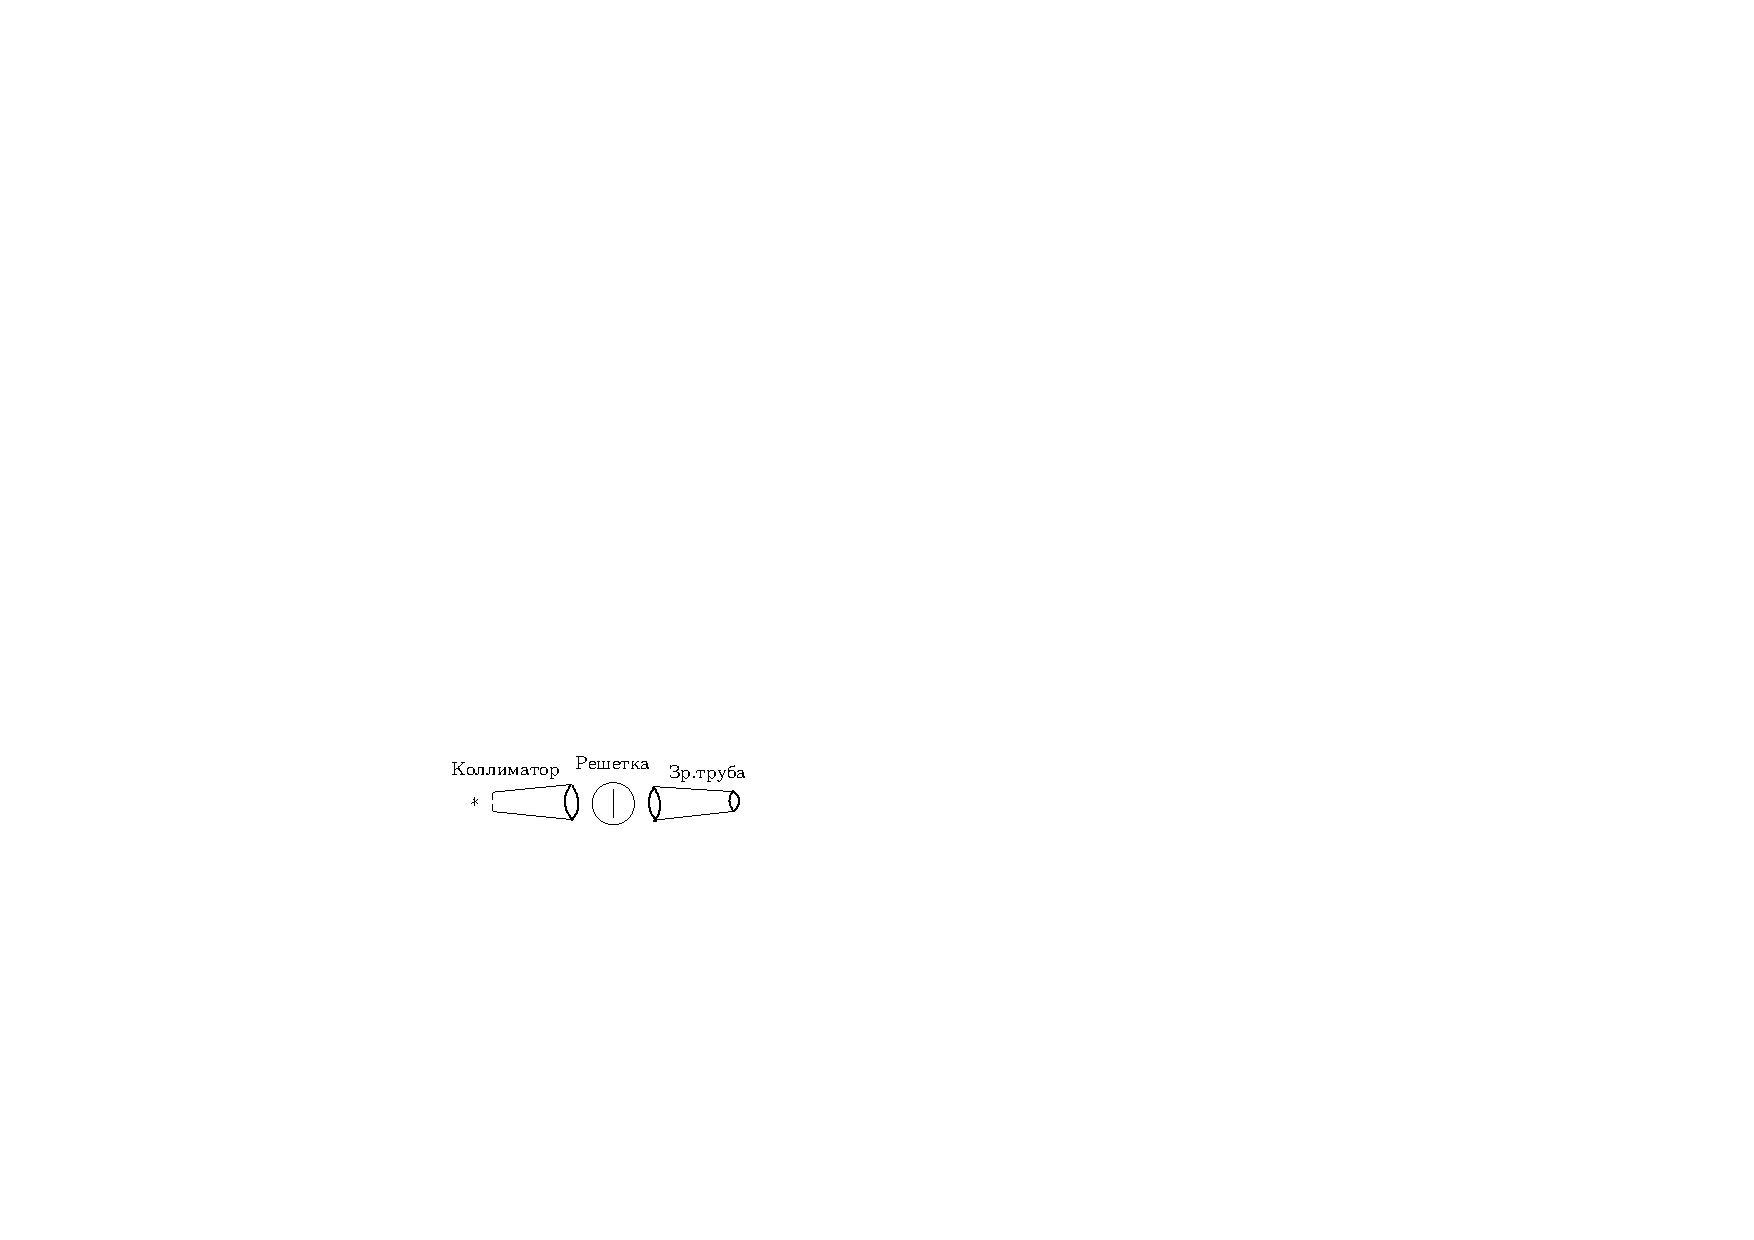
\includegraphics[scale=1.5]{inst.pdf}
	\end{center}
	\caption{Схема установки}
\end{figure}

\section{Ход работы}

Измерим угловые координаты спектральных линий ртути в $ \pm1 $ порядках, рассчитаем углы дифракции $\varphi_m$. Результаты измерений и вычислений занесем в таблицу~\ref{table:exp1}.
		\begin{table}[H]
			\caption{Измерение угловых положений спектральных линий}
			\label{table:exp1}
			\begin{center}
			    \begin{tabular}{|p{2.2cm}|p{1.5cm}|p{1.5cm}|p{1.5cm}|p{1.5cm}|p{1.5cm}|p{1.5cm}|p{1.5cm}|}
				\hline
				 & синий  & голубой & зеленый & желтый & желтый & красный & красный \\ \hline
				$ \varphi $&  $12^{\circ}34'55'' $& $14^{\circ}13'44''$ & $15^{\circ}50'49'' $& $16^{\circ}45'51'' $& $16^{\circ}49'45''$ & $17^{\circ}49'58'' $& $18^{\circ}09'50''$ \\ \hline
				$\sin \varphi$   & 0,2178 & 0,2457  & 0,2731  & 0,2884 & 0,2895 & 0,3062  & 0,3117  \\ \hline
				$ \lambda $, нм   & 435,8  & 491,6   & 546,1   & 577,0    & 579,1  & 623,4   & 690,7   \\ \hline
			\end{tabular}
			\end{center}
			
		\end{table}
		Для оценки угловой дисперсии решётки определим разности угловых координат линий жёлтого дублета во всех видимых порядках ($ \Delta \lambda = 21  \buildrel _{\circ} \over {\mathrm{A}} $):

		\begin{table}[H]
    \centering
    \begin{tabular}{|c|c|c|c|}
    \hline
    m  & $\Delta\varphi, ''$  & $D\cdot10^{-5}$ рад/$\buildrel _{\circ} \over {\mathrm{A}}$    & $\sigma_D\cdot10^{-5}$ рад/$\buildrel _{\circ} \over {\mathrm{A}}$ \\ \hline
    1  & 224  & 5.17   & 0.21  \\ \hline
    -1 & 239  & -5.52  & 0.22  \\ \hline
    2  & 588  & 13.57  & 0.54  \\ \hline
    -2 & 548  & -12.65 & 0.51  \\ \hline
    3  & 1350 & 31.17  & 1.25  \\ \hline
    -3 & 1332 & -30.75 & 1.23  \\ \hline
    \end{tabular}
    \caption{Исследование угловой дисперсии}
    \label{tab:disp}
\end{table}
	
	\section{Обработка результатов}
	Построим график зависимости $\sin \varphi_m$ от длины волны $\lambda$ для $\pm 1$ порядка:
	
	\begin{center}
	\begin{tikzpicture}
	\begin{axis}[
	title={График 1 \quad График зависимости угловой координаты спектральных линий от длины волны},
	xlabel={$\lambda$, мм},
	ylabel={$\sin\phi_m$},
	legend pos=north west,
	xmajorgrids=true,
	ymajorgrids=true,
	grid style=dashed,
	width = 520,
	height = 300,
	%xmin = 300,
	%xmax = 335,
	%ymin =40,
	%ymax =0.22,
	]
	\legend{ 
		Результат измерений,
		Аппроксимация
	};
	\addplot+ [blue, only marks, mark size = 4pt,
	error bars/.cd,
	x dir=both, x explicit,
	y dir=both, y explicit, 
		] table [x = T, y = sigma, y error = dy] {
		T	sigma               dy
		690.7	0.321735775     0.01
        623.4	0.306237265     0.01
        579.1	0.289516478     0.01
        577	    0.288432752     0.01
        546.1	0.273065987     0.01
        491.6	0.245793652     0.01
        435.8	0.217833218     0.01

	};
	\addplot [red, domain=420:700, line width =3.2pt] {x*3.90402*10^-4 + 0.05614};
	\end{axis}
	\end{tikzpicture}
\end{center}
	
	    Определим по углу наклона графика период решётки $d$:
	    \begin{equation}
			1/d = (453\pm21) \ \text{штрих/мм}
		\end{equation}
		
		\begin{equation}
			d = (2,2\pm 0,1) \ \text{мкм}
		\end{equation}
	
	    Для угловой дисперсии построим график зависимости этой величины от порядка дифракции.
	    
\begin{center}
	\begin{tikzpicture}
	\begin{axis}[
	title={График 2 \quad График зависимости угловой дисперсии от порядка максимума},
	xlabel={$m$},
	ylabel={$D$, рад/А},
	legend pos=north west,
	xmajorgrids=true,
	ymajorgrids=true,
	grid style=dashed,
	width = 520,
	height = 300,
	%xmin = 300,
	%xmax = 335,
	%ymin =40,
	%ymax =0.22,
	]
	\legend{ 
		Результат измерений,
		Теоретическая зависимость
	};
	\addplot+ [blue, only marks, mark size = 4pt,
	error bars/.cd,
	x dir=both, x explicit,
	y dir=both, y explicit, 
	] table [x = T, y = sigma] {
		T	sigma
		1	0.000051713459
        -1	-0.000055176414
        2	0.00013574783
        -2	-0.00012651328
        3	0.00031166594
        -3	-0.00030751039
	};
	\addplot [red, domain=-3.2:3.2, line width =3.2pt] {x/(21000^2-x^2*5780.5^2)^0.5};
	\end{axis}
	\end{tikzpicture}
\end{center}
	    
		Оценим разрешимый спектральный интервал $ \delta\lambda $, разрешающую способность $ R $ и число эффективно работающих штрихов решётки $ N $, а также её эффективный размер $ l $. По результатам измерений угловая ширина первой жёлтой линии составляет $\Delta\varphi = 30''$.
		\begin{equation}
			\delta\lambda \approx \Delta\varphi/D = (2.8 \pm 0.2) \buildrel _{\circ} \over {\mathrm{A}};
		\end{equation}
		\begin{equation}
			R \approx \frac{\lambda}{\delta\lambda} = 2055 \pm 146 
		\end{equation}
		\begin{equation}
			N \approx R/m = 2055 \pm 146
		\end{equation}
		\begin{equation}
			l \approx Nd = (4.5 \pm 0.3)\; \text{мм}
		\end{equation}
		
Найдём порядок дифракции при которой жёлтая линия спектра совпадёт с фиолетовой:

\[(m+1)\lambda_\text{ф}=m\lambda_\text{ж}\]
\[m=\frac{\lambda_\text{ф}}{\lambda_\text{ж}-\lambda_\text{ф}}\approx3.1\]

\section{Обсуждение результатов и выводы}
В ходе выполнения лабораторной работы были получены следующие результаты.
\begin{itemize}
    \item Экспериментально измерено положение спектральных линий ртутной лампы в $\pm$ 1 порядке. По полученным данным был вычислен период дифракционной решётки.
    \[1/d=(453\pm 21) \ \text{штрих/мм}\]
    \[\boxed{d = (2.2\pm 0.1) \ \text{мкм}}\]
    Эти данные примерно совпадают с реальными параметрами решётки $1/d = 500\ \text{штрих/мм}$.
    \item Далее была исследована угловая дисперсия дифракционной решётки, её зависимость от порядка максимума. Для жёлтой пары она была измерена в 3 порядках. Результаты представлениы на Графике 2. Экспериментальные данные хорошо описывают теоретическую зависимость.
    \item По результатам измерений были определены основные параметры дифракционной решётки для первого порядка дифракции. Была определена разрешающая способность, эффективное число штрихов и её эффективный размер.
    \[\boxed{R = 2055 \pm 146}\]
    \[\boxed{N = 2055 \pm 146}\]
    \[\boxed{l \approx Nd = (4.5 \pm 0.3)\; \text{мм}}\]
    \item Также был рассчитан порядок дифракции при которой жёлтая линия спектра совпадёт с фиолетовой.
    \[\boxed{m=3.1}\]
\end{itemize}

Результаты, полученные в ходе выолнения работы можно назвать удовлетворительными. Основной вклад в погрешность вности неточность опредения цвета той или иной спектральной линии в силу слабой интенсивности некоторых линий спектра. Также свой вклад вности неточность, появляющаяся в результате некоторого смещения нуля отсчёта угловых координат гониометра.
\end{document}